\documentclass[ngerman, a4paper, footsepline, headsepline, numbers=noenddot]{scrreport}
\usepackage[T1]{fontenc}
\usepackage[utf8]{inputenc}
\usepackage{babel, lmodern, scrlayer-scrpage, amsmath, amsmath, amsfonts, graphicx, tikz}
\usepackage[bottom=5cm]{geometry}

\pagestyle{scrheadings}
\pagenumbering{Roman}
\newcommand{\myifoot}{\textbf{Emanuel Schäffer}}
\newcommand{\mychead}{\textbf{RWU--University of Applied Sciences}}
\automark{section}
\ofoot{\headmark}
\ohead{\today}
\chead{\mychead}
\ifoot{\myifoot}

\newcommand{\figref}[1]{(siehe Abb.~\ref{#1})}

\newenvironment{myenv}{%
	\begin{center}
}{%
	\end{center}
}

\begin{document}
	\subject{Kryptoanalyse der Enigma-Maschine: Eine Untersuchung des Cyclometers und der Turing-Bombe}
	\title{Kryptoanalyse der Enigma-Maschine}
	\author{Emanuel Schäffer}
	\date{\today}
	\publishers{RWU--University of Applied Sciences}
	\maketitle
	
	\begin{abstract}
		Enigma-Nachrichten können dechiffriert werden, wenn die Rotorauswahl\footnote{Hier wird im Allgemeinen nur die Enigma M1 mit 5 Walzen betrachtet.}, die Rotor-~, Ringstellungen und die Steckereinstellungen einzeln wiederhergestellt werden. Die Wiederherstellung der Nachrichtenschlüsseleinstellung ist empfindlich genug, um die korrekte Rotorreihenfolge zu unterscheiden. Die Methode wird an einer 647 Zeichen langen Nachricht demonstriert und ihre Leistung für unterschiedliche Nachrichtenlängen und verwendete Steckeranzahlen geschätzt.
	\end{abstract}


	\chapter{Enigma}
	
	Die Enigma ist eine Rotor-Chiffriermaschine, die hauptsächlich im Zweiten Weltkrieg Einsatz kam. Die von der Wehrmacht modifizierte Enigma verfügte zunächst über drei Walzen und zusätzlich einen Reflektor. Jede dieser Walzen führte eine monoalphabetische Substitution durch. Die rechte Walze wurde bei jedem Tastendruck um eine Position weitergerückt. Hat diese Walze eine komplette Rotation vollzogen, rückte die Walze links neben ihr um eine Position weiter\footnote{Eine Analogie hierfür ist der Kilometerzähler eines mechanischen Tachometers oder das Verhalten von Sekunden-, Minuten- und Studenzeigern einer Uhr.}. Neuerungen waren das Steckerbrett \figref{fig:enigma_complete} und gegen Ende des Krieges eine zusätzliche, vierte Walze. Ich werde mich, wenn nicht ausdrücklich erwähnt, auf die Enigma M3 mit drei Walzen beschränken.
	\nopagebreak
	\begin{figure}[htbp]
		\centering
		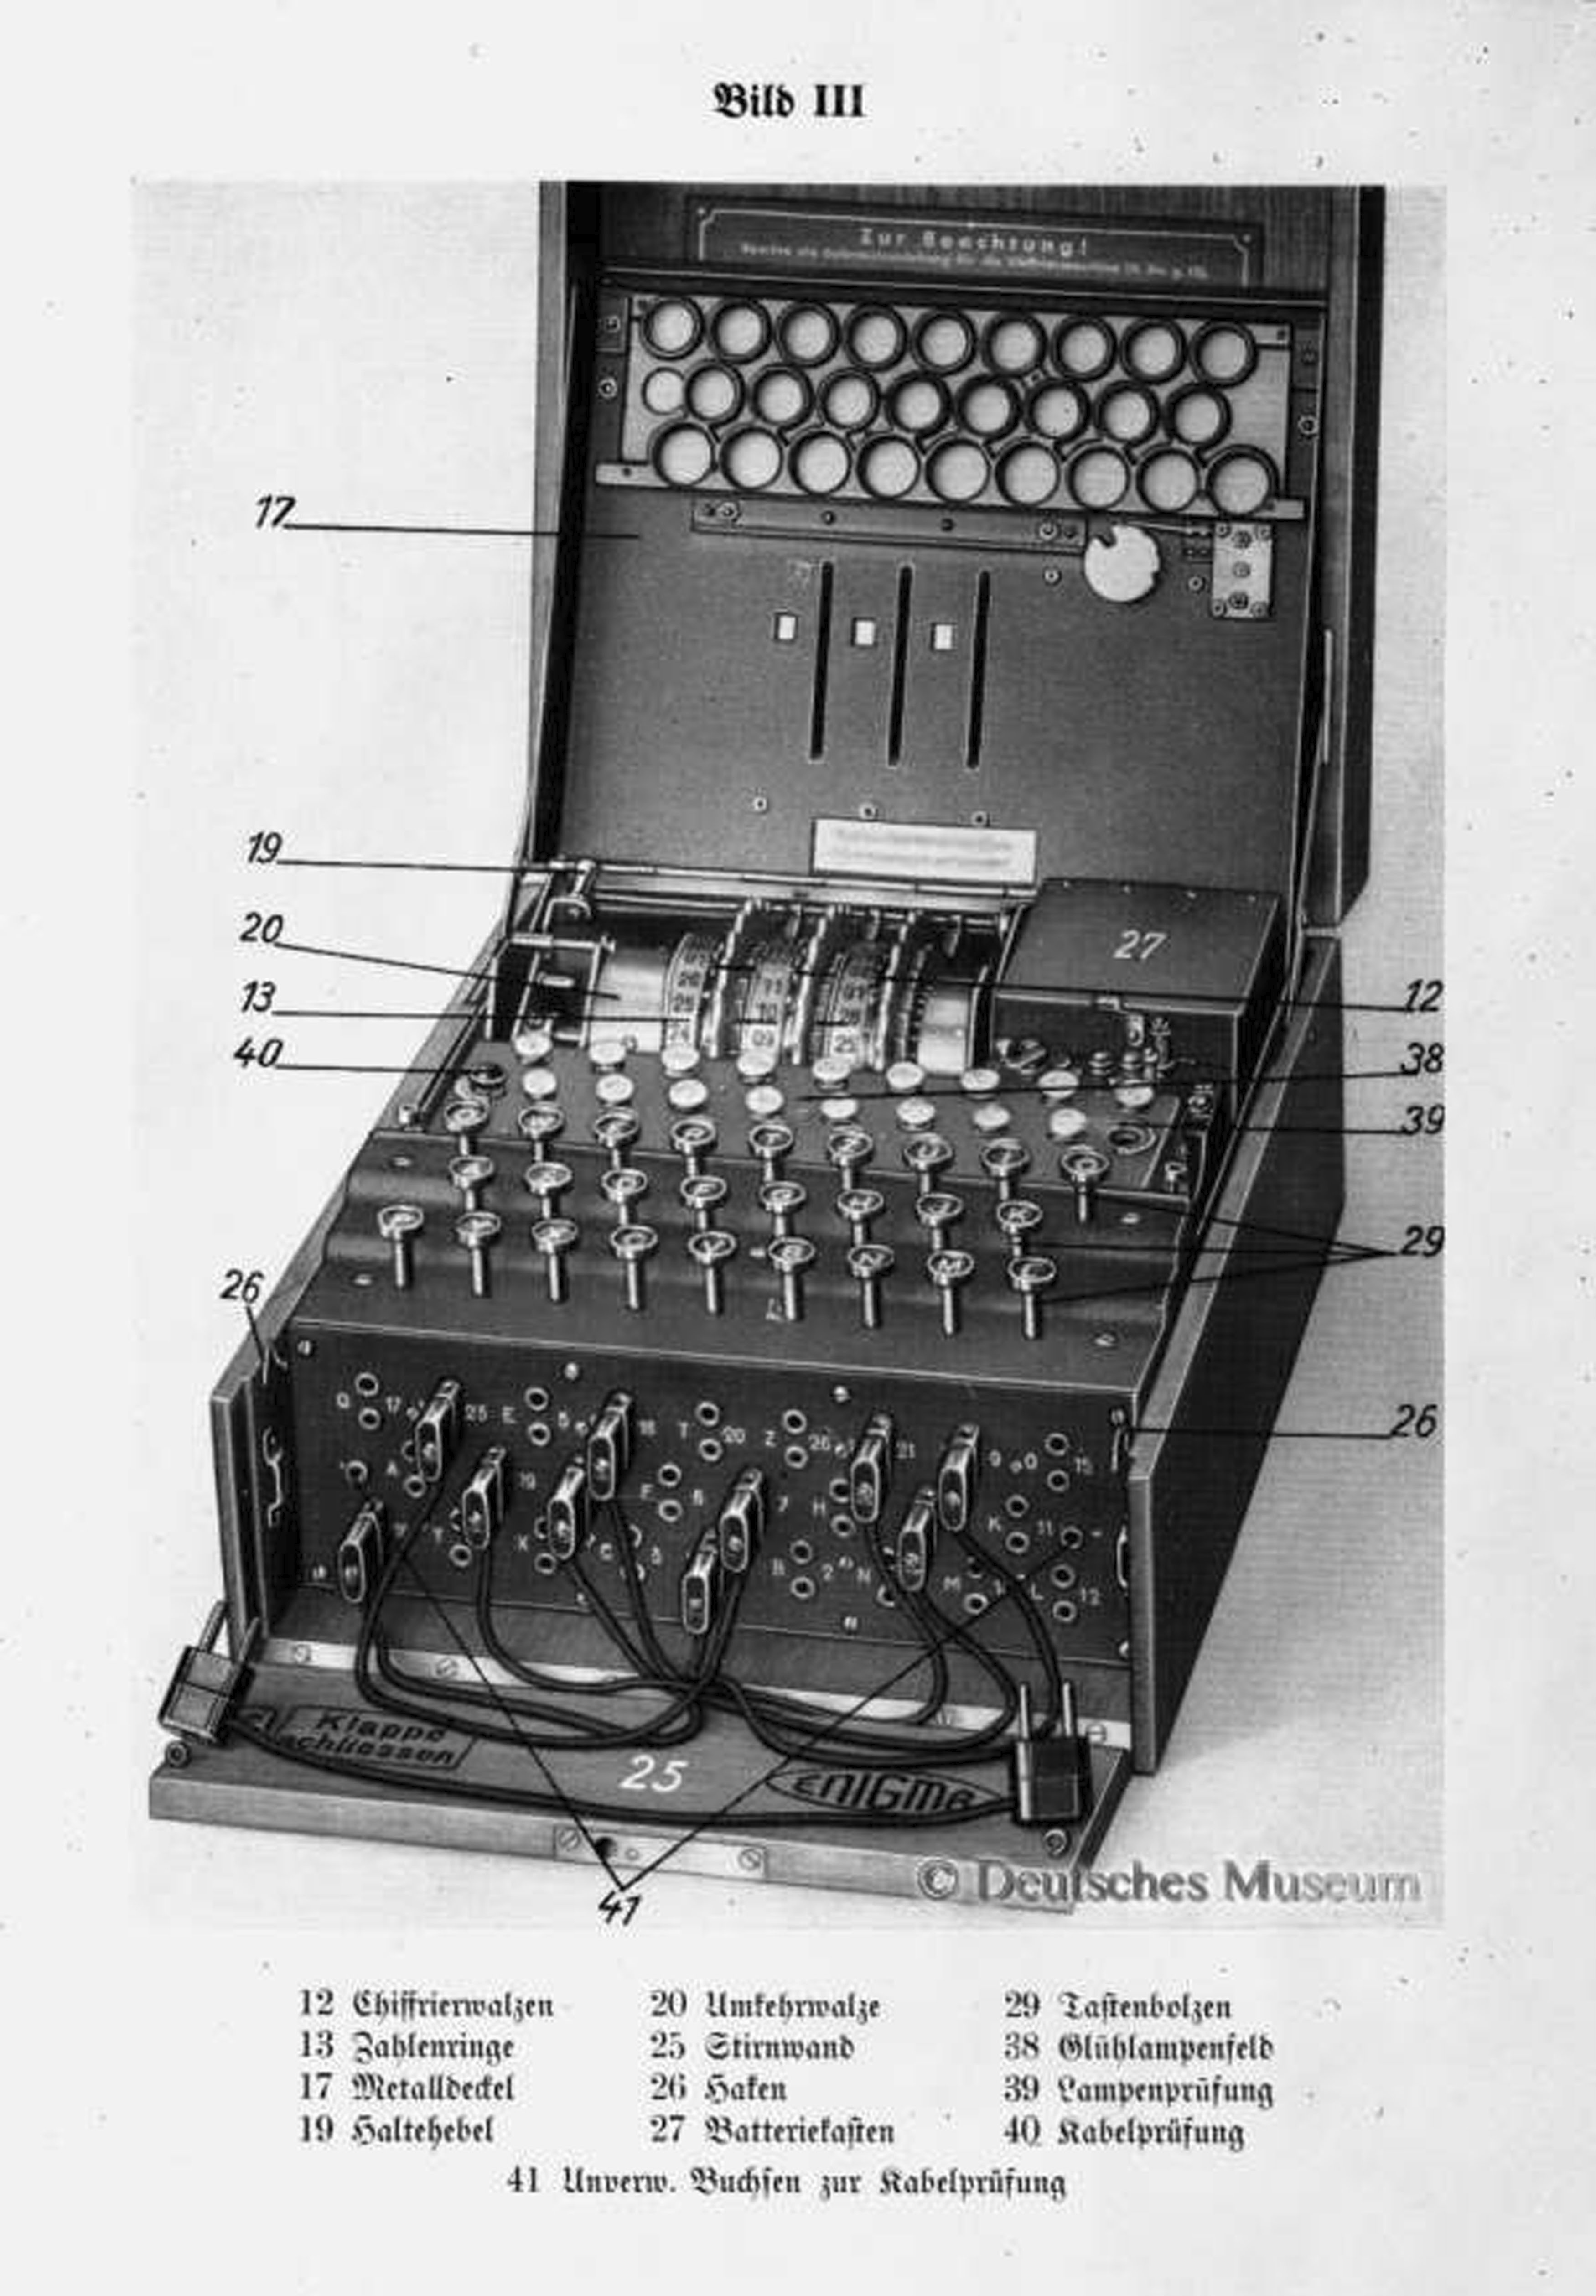
\includegraphics[width=.5\linewidth]{Enigma-komplett.png}
		\caption{Die Enigma Maschine}
		\label{fig:enigma_complete}
	\end{figure}
	
	\newpage
	
	 Bei der Enigma wurde jeden Tag  eine Tagesschlüssel eingestellt, welcher durch ein Code-Buch vorgegeben war. Dieser Tagesschlüssel bestand darin, welche drei der fünf Walzen der Schlüssler in welcher Reihenfolge einzusetzen hatte. Ferner musste er die Walzenstellung einstellen. Sie bestimmt die Ausgangsstellung der Walzen. Diese konnte durch ein Sichtfenster abgelesen werden.
	
	\begin{figure}[htbp]
		\centering
		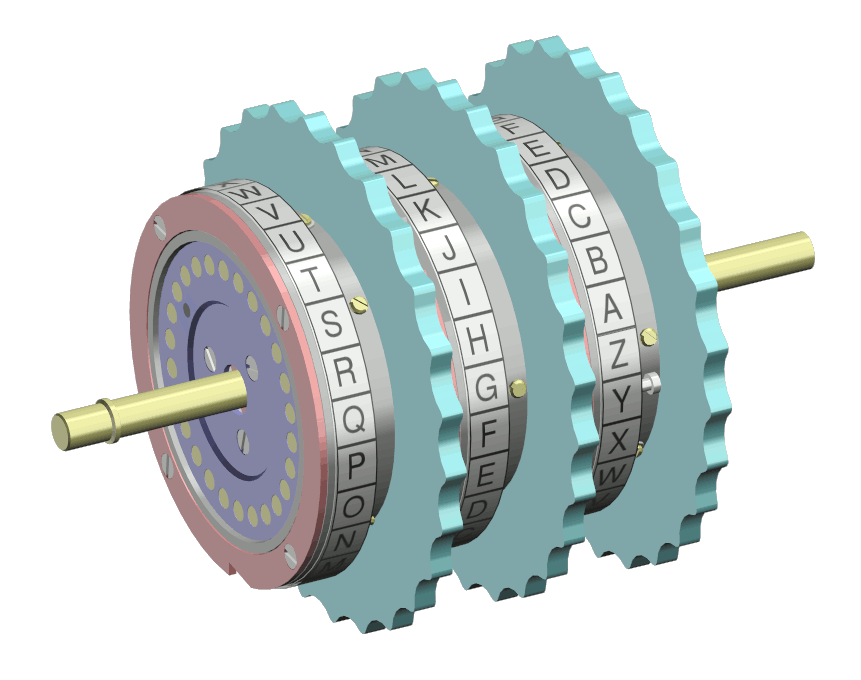
\includegraphics[width=.4\linewidth]{Enigma-rotor-set.png}
		\caption{Enigma-Walzen}
		\label{fig:enigma_rotors}
	\end{figure}
	
	Zusätzlich musste der Schlüssler die Ringstellung des Tages einstellen. Die Ringstellung veränderte die Relation der sichtbaren Buchstaben mit der internen Verdrahtung und bewegte die Übertragskerbe \figref{fig:enigma-rotor-contact}, die festlegte, wann sich die Walze links von der aktuellen bewegt.
	
	\begin{figure}[htbp]
		\centering
		\begin{tikzpicture}
			\node at (0,0) {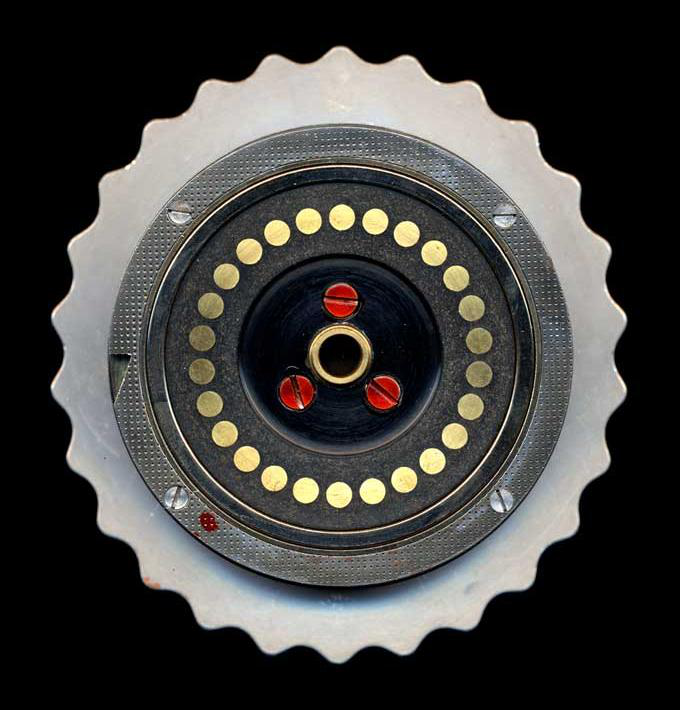
\includegraphics[width=.3\linewidth]{Enigma-rotor-flat-contacts.png}};
			\draw[red, very thick, ->] (-3,-0.5) -- (-1.5,-0.1) ;
			\node[red, anchor=west] at (-5,-0.8) {Übertragskerbe};
		\end{tikzpicture}
		\caption{Walzen Frontansicht mit Übertragskerbe}
		\label{fig:enigma-rotor-contact}
	\end{figure}
	
	\newpage
	Als letzte Einstellung musste das Steckerbrett verdrahtet werden. Das Steckerbrett vertauschte zwei Buchstaben miteinander. Von 13 möglichen Steckerverbindungen wurden meistens 10 vorgegeben. Nachdem alle Einstellung getroffen waren, überlegte sich der Schlüssler einen "`zufälligen"' Spruchschlüssel, mit dem der Text verschlüsselt wurde.\footnote{In Wahrheit wählten die Schlüssler oft den gleichen Schlüssel, der meist persönliche Informationen wie zum Beispiel den Name der Freundin enthielt.} Dieser Spruchschlüssel gab die Walzenstellung für die folgende Nachricht an. Der "`zufällige"' Spruchschlüssel wurde mit dem Tagesschlüssel verschlüsselt und ergab zusammen mit anderen Zusatzinformationen den "`Spruchkopf"'. Der Schlüssler gab nun den zu verschlüsselnden Text nach bestimmten Regeln ein. Eine Eigenschaft der Enigma ist, dass sie selbstinvers ist. Das bedeutet, dass mit der gleichen Einstellung, mit der ein Text verschlüsselt wurde, dieser auch wieder entschlüsselt werden kann.
	
	
	\chapter{Häufigkeitsanalyse}
	\section{Koinzidenzindex}
	\thispagestyle{scrheadings}
	
	Zunächst benötigen wir ein geeignetes Maß, um den Grad der Annäherung eines teilweise dechiffrierten Klartextes an authentisches Deutsch abzuschätzen. Dafür verwenden wir den Koinzidenzindex:
	
	$$
	IC = \frac{\sum_{i=A}^{Z}f_i(f_i-1)}{N(N-1)}
	$$
	
	Sei $f_i$ die Häufigkeit des Buchstabens in Abhängigkeit von $i$ und $N$ die Gesamtanzahl der Buchstaben. Wir Summieren also die Anzahl der Buchstabenpaare auf, und teilen diese durch die Anzahl der allgemein möglichen Buchstabenpaare. Der Koinzidenzindex ist also ein Maß für die Buchstabenverteilung. Für ein Text bestehend aus zufälligen Buchstaben beträgt der $IC \approx$ 0.038; wobei er für Deutsch $\approx$ 0.076 beträgt.
	\newpage
	
	Bemerkungen:
	
	Improvements:
	
	Base: 8.5s
	
	Nur letzte Buchstaben testen: 3.6s
	
	IC: 3.3s
	
	Low Level IO: 3.31s
	
	Nur erster char testen an der Position, an dem das Schlagwort stehen muss: 2.25s 
	
	
	\chapter{Quellen}
	
	%Deutsches Museum, Ertl Angewandte Kryptographie \ref{fig:enigma_complete}
	
	%https://upload.wikimedia.org/wikipedia/commons/9/9f/Enigma_rotor_set.png Zugriff %11.09.24. 10:57 \ref{fig:enigma_rotors}
	
	%https://de.wikipedia.org/wiki/Enigma-Walzen#/media/Datei:Enigma-rotor-flat-contacts.jpg Zugriff 11.09.24. 11:19 \ref{fig:enigma-rotor-contact}
	
	
	
\end{document}